% !TEX root = main.tex
\label{ch:pilot-data-hadoop}

Computational campaigns on High Performance Computing (HPC) resources can execute compute- or data- intensive workflows and applications.
On one hand, compute-intensive applications and workflows are associated with either a single long running executable or an ensemble of compute-intensive tasks~\cite{balasubramanian2018harnessing}.
On the other hand, data-intensive applications are associated with multiple stages of execution which can be I/O, memory and compute bound.
While MPI is the most common programming model for compute-intensive applications, the MapReduce~\cite{dean2004mapreduce} abstraction is commonly used for data-intensive applications~\cite{hellerstein2012science}.

%However, HPC resources are designed to support mainly compute-intensive long-running MPI applications, as they offer
%Not surprisingly, HPC resource architectures offer large number of computing resources, e.g., CPUs and GPUs, connected by high-end networks (e.g., Infiniband) and filesystems, such as Lustre and PVFS.
%They have however limitations in supporting data-intensive and I/O bound workflows.

Hadoop~\cite{hadoop} popularized the use of MapReduce~\cite{dean2004mapreduce} for data-intensive applications.
Hadoop's distirbuted filesystem (HDFS) automatically partitions data and distributes them to different nodes of a cluster machine.
In addition, Hadoop's engine takes advantage of data-locality and transfers computations to nodes, allowing to process data in parallel while reducing data transfers.
While Hadoop simplified the processing of vast volumes of data, it has limitations in its expressiveness~\cite{yelick2011magellan,isard2007dryad}.
The complexity of creating sophisticated applications such as, for example, iterative machine learning algorithms \mtnote{add a reference here?}, required multiple MapReduce jobs and persistence to Hadoop's Filesystem (HDFS) after each iteration.
This led to devise several higher-level abstractions and the development of processing frameworks to implement sophisticated data pipelines.

Spark~\cite{zaharia2010spark} is the most well-known processing framework in the Hadoop ecosystem.
In contrast to MapReduce, Spark provides a richer API, more language bindings and a memory-centric processing engine that can utilize distributed memory and retain resources across multiple task generations.
Spark's \emph{Reliable Distributed Dataset (RDD)} ~\cite{zaharia2012resilient} abstraction provides a powerful way to manipulate distributed collections stored in cluster nodes' memory.
Spark is used to build complex data workflows and advanced analytic tools, such as MLLib~\cite{mllib}.
Although the addition/development of new and higher-level execution frameworks addressed some of the problems of data processing, it introduced the problem of heterogeneity of access and resource management.

% Problem statement.
Some computational campaigns cannot be easily classified as only compute- or data-intensive. For example, the simulations of contemporary bio-molecular dynamics~\cite{dror2012biomolecular} campaigns require increasing time scales and problem sizes,  generating amounts of data several order of magnitude larger than those so far generated. Further, data generated by those simulations often need to be analyzed so as to determine the next set of simulation configurations.
Several tools evolved to meet the demand for molecular dynamics data analysis, such as MDAnalysis~\cite{michaud2011mdanalysis,gowers2016mdanalysis}, CPPTraj~\cite{roe2013ptraj} and HiMach~\cite{tiankai2008scalable}.
Although these tools offer domain-specific analytics, scaling them to high data volumes remains a challenge, especially when the scale of teh computation erquires the use of high performance computing (HPC) infrastructures.
This is therefore a need for computing environments that support scalable data processing while preserving the ability to run simulations at large scale.
To the best of our knowledge, there does not exist a solution that provides the integrated capabilities of Hadoop and HPC.

% Solution
In this chapter, we explore the integration between Hadoop~\cite{hadoop}, Spark~\cite{zaharia2010spark} and HPC resources.
We utilize the Pilot-Abstraction~\cite{luckow2012pstar}, allowing to manage HPC and data-intensive applications in a uniform way.
We explore two extensions to RADICAL-Pilot~\cite{merzky2018design}, a Pilot-Job~\cite{luckow2012pstar} runtime system designed for implementing task-parallel applications on HPC: 
\begin{inparaenum}[1)]
    \item the ability to spawn and manage Hadoop/Spark clusters on HPC infrastructures on demand (Mode I); and
    \item to connect and utilize Hadoop and Spark clusters for HPC applications (Mode II)
\end{inparaenum}.
Both extensions facilitate the application and resource management requirements of data-intensive applications.
By supporting these two usage modes, RADICAL-Pilot simplifies the barrier of deploying and executing HPC and Hadoop/Spark workflows side-by-side.

The chapter is organized as follows: In section~\S\ref{sec:hpc_hadoop_rel} we discuss the current solutions and challenges of integrating data analytics and HPC.
We continue with discussing the modes of integration and interoperability between data analytics and HPC in~\S\ref{sec:integration_mode} and the experimental validations of the integration in~\S\ref{sec:rph-exps}.
The chapter closes with our conclusions in section~\S\ref{sec:hpc_hadoop_concl}.

\section{Related Work and Challenges}
\label{sec:hpc_hadoop_rel}
%\subsection{Related Work}

There are several frameworks which explored the usage of Hadoop on HPC resources, e.g., Hadoop on Demand~\cite{hod}, JUMMP~\cite{moody2013jummp}, MagPie~\cite{chu2015magpie}, MyHadoop~\cite{krishnan2011myhadoop} and MyCray~\cite{mycray}.
These frameworks provide users with a set of scripts that can spawn and manage an Hadoop cluster on HPC resources.
As soon as Hadoop is started, users can either submit their MapReduce jobs interactively or via a script.

Although these frameworks can spawn and manage Hadoop clusters, they isolate the Hadoop cluster from the HPC environment.
The scripts and capabilities they offer interact directly with the HPC's submission system.
As a result, users cannot execute on the same set of nodes HPC and Hadoop applications.
Further, they do not necessarily optimize configurations and resource usage, including the use of available SSDs, parallel filesystems and high-end network features, e.g., RDMA~\cite{rahman2014homr}.

%\subsection{Challenges}
Hadoop originally provided a rudimentary resource management system, the YARN scheduler.
The YARN scheduler~\cite{vavilapalli2013apache} provides an application-level scheduling framework addressing the increased requirements with respect to applications and infrastructure, such as more complex data localities (memory, disk, datacenter), long-lived services, periodic jobs, interactive and batch jobs.
In contrast, to batch schedulers of HPC resources, YARN is optimized for supporting data-intensive environments and managing a large number of fine-grained tasks.

While YARN manages system-level resources, applications need to implement an application-level scheduler that optimizes their specific requirements, e.g., with respect to data locality.
This application-level scheduler, the \textit{Application Master}, is responsible for allocating resources---called containers---and executing tasks on these resources.
In addition, the Application Master manages data locality, e.g., between HDFS blocks and container locations, by allocating containers on specific nodes.

Managing resources on top of YARN is associated with several challenges.
While applications with fine-grained, short-running tasks are well supported, applications with coarse-grained, long-running task, such as MPI applications, are not.
To achieve interoperability and integration between Hadoop and HPC, it is essential to consider a more diverse set of applications on top of YARN.

A particular challenge for Hadoop on HPC deployment is the choice of storage and filesystem backend.
Typically, when using Hadoop local storage is preferred.
Nevertheless, in some cases, e.g., processing many small files, random data access is required or the number of parallel tasks is low to medium, using a parallel filesystem can yield a better performance.
For this purpose, many parallel filesystems provide a special client library which improves the interoperability with Hadoop, but limits data locality and any data placement optimization.

Another challenge is the integration between both HPC and Hadoop environments.
Rather than preserving HPC and Hadoop ``environments'' as software silos, there is a need for an approach that integrates them. 
We utilize the Pilot-Abstraction as a unifying concept to efficiently support the integration, and not just the interoperability between HPC and Hadoop.
By utilizing the multi-level scheduling capabilities of YARN, the Pilot-Abstraction can efficiently manage Hadoop resources providing an application with the means to reason about data, compute resources and allocation.
In addition, we show how the Pilot-Abstraction can be used to manage Hadoop applications on HPC environments.

The Pilot-Abstraction~\cite{luckow2012pstar} is successfully used on HPC resources supporting a diverse set of task-based workflows.
A Pilot-job is a placeholder job which is submitted to the resource management system and represents a container for a dynamic set of tasks.
Pilot-jobs are, also, a well-known example of multi-level scheduling, which is often used to separate system-level resource and user-level workload management.
The Pilot-Abstraction defines the following entities:
\begin{inparaenum} [1)]
    \item a Pilot which allocates a set of computational resources (e.g., cores); and
    \item  a Compute-Unit (CU) as a self-contained piece of work represented as an executable.
\end{inparaenum}
The Pilot-Abstraction has been implemented within RADICAL-Pilot~\cite{merzky2018design}.


\section{Data analytics and HPC integration: RADICAL-Pilot and YARN/ Spark}
\label{sec:integration_mode}
Having established the potential of the Pilot~-Abstraction for a range of high-performance applications~\cite{treikalis2016repex,ragothaman2014developing,ko2014numerical}, we use it as the starting point for integrating HPC and data-intensive analytics.
As depicted in Figure~\ref{fig:figures_hadoop-on-hpc-viceverse}, there are at least two different usage modes to consider:
\begin{inparaenum}[1)]
    \item Mode I: Running Hadoop/Spark applications on HPC environments (Hadoop on HPC),
    \item Mode II: Running HPC applications on YARN clusters (HPC on Hadoop).
\end{inparaenum}

\begin{figure}[t]
    \centering
    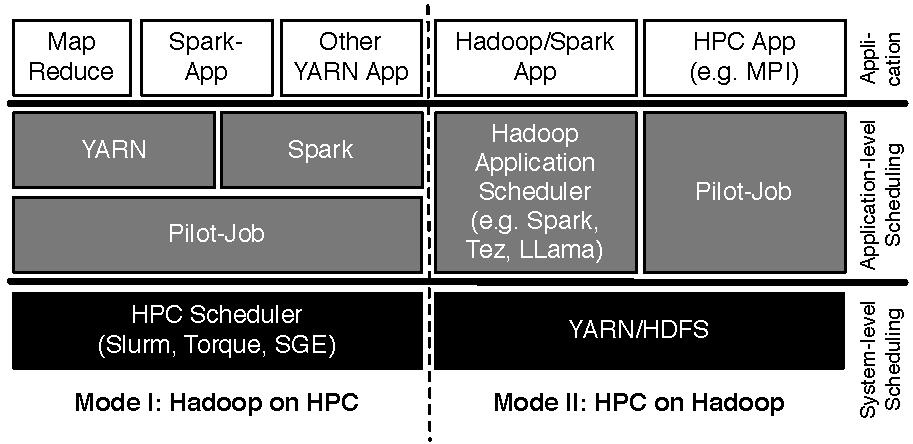
\includegraphics[width=.85\textwidth]{figures/data_analytics_hpc/hpc_hadoop/hadoop-on-hpc-viceverse.pdf}
    \caption{Hadoop and HPC Interoperability modes\label{fig:figures_hadoop-on-hpc-viceverse}}
\end{figure}

Mode I is critical to support traditional HPC environments so as to support applications with both compute and data requirements.
Mode II is important for cloud environments (e.g., Amazon's Elastic MapReduce) and an emerging class of HPC machines with new architectures and usage modes, such as Wrangler~\cite{wrangler}, that support Hadoop natively.
For example, Wrangler supported dedicated Hadoop environments (based on Cloudera Hadoop 5.3) via a reservation mechanism.
%We discuss, the integration of Hadoop and Spark runtimes into RADICAL-Pilot, which enables both the interoperable use of HPC and Hadoop, as well as the integration of HPC and Hadoop applications (Mode I and II).
Using these new capabilities, applications can seamlessly connect HPC stages (e.g., simulation stages) with analysis staging using the Pilot-Abstraction to provide unified resource management.
%\subsection{Mode I---II: }
%\label{ssec:rp-impl}

With the introduction of YARN, a broader set of applications can be executed within a Hadoop cluster than earlier.
However, developing and deploying YARN applications potentially side-by-side with HPC applications remains a difficult task.
Established abstractions which are easy to use while enabling users to reason about compute and data resources across infrastructure types (i.e., Hadoop, HPC and clouds) are missing. 

Schedulers such as YARN effectively facilitate application-level scheduling.
Although, the development efforts for YARN applications are still high.
YARN provides a low-level abstraction for resource management, e.g., a Java API and protocol buffer specification.
Typically interactions between YARN and applications are much more complex than the interactions between an application and an HPC scheduler.
Further, applications must be able to run on a dynamic set of resources; YARN e.g., can preempt containers in high-load situations.
Data/compute locality need to be manually managed by the application scheduler by requesting resources at the location of a file chunk.
Also, the scheduler can preempt resources (the so called YARN containers).

To address these shortcomings, various frameworks that aid the development of YARN applications have been proposed.
Llama~\cite{llama} offers a long-running application master for YARN designed for the Impala SQL engine.
Apache Slider~\cite{apache-slider} supports long-running distributed application on YARN with dynamic resource needs allowing applications to scale to additional containers on demand.
While these frameworks simplify development, they do not address concerns such as interoperability and integration of HPC/Hadoop.
Integrating YARN and RADICAL-Pilot (RP) allows applications to run HPC and YARN applications on HPC resources concurrently.

\subsubsection*{RADICAL-Pilot and YARN Overview}
\label{sssec:rp_yarn}
% RADICAL-Pilot Overview
Figure~\ref{fig:comp_rp_arch} illustrates the architecture of RADICAL-Pilot and the components that were extended.
The figure on the left shows the macro architecture of RADICAL-Pilot.
The figure on the right shows the architecture of the Pilot-Agent which is a critical functional component.
RADICAL-Pilot consists of a client module with the Pilot-Manager and Unit-Manager and a set of RADICAL-Pilot-Agents running on resources.
The Pilot-Manager is the central entity responsible for managing a set of pilots.
Pilots are described via a Pilot description, which contains the pilot's resource requirements and is submitted to the Pilot-Manager.
The Pilot-Manager, then, submits a placeholder job which will run the RADICAL-Pilot-Agent via the Resource Management System using the SAGA-API~\cite{merzky2015saga} (steps P.1-P.2).
Subsequently, the Unit-Manager and the RADICAL-Pilot-Agent manage the application workload (the Compute-Units,steps U.1-U.7)~\cite{merzky2019using}.

\begin{figure}
    \centering
    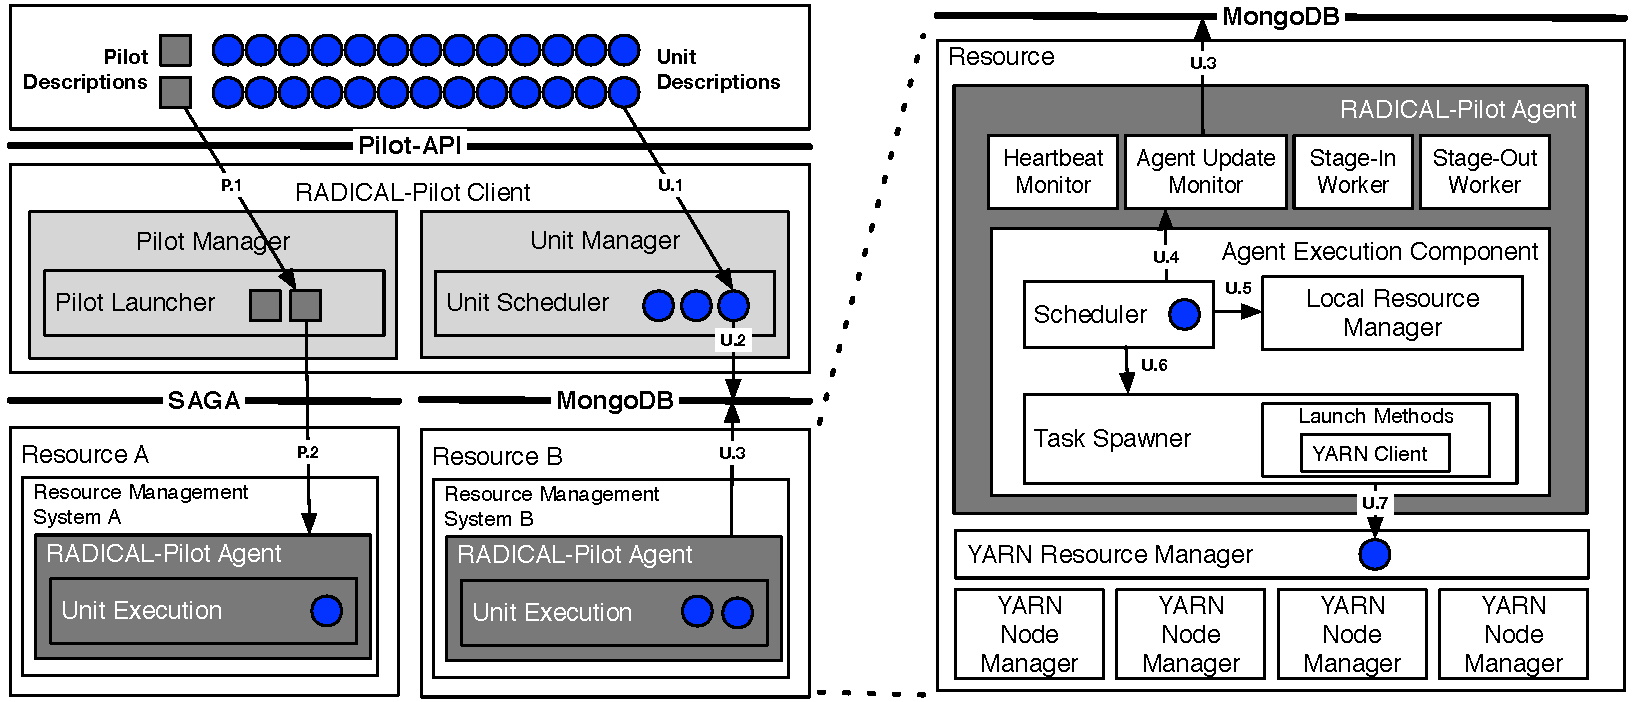
\includegraphics[width=0.85\textwidth]{figures/data_analytics_hpc/hpc_hadoop/rp-architecture-yarn.pdf}
    \caption{\textbf{RADICAL-Pilot and YARN Integration:} There are two main interactions between the application and RADICAL-Pilot---the management of Pilots (P.1--P.2) and the management of Compute Units (U.1-U.7).  All YARN specifics are encapsulated in the RADICAL-Pilot-Agent.\label{fig:comp_rp_arch}}
\end{figure}

The RADICAL-Pilot-Agent has a modular and extensible architecture and consists of the following components: the Agent Execution Component, Heartbeat Monitor, Agent Update Monitor, Stage In and Stage Out Workers.
The main integration of YARN and RP is done in the Agent Execution Component.
This component consist of four sub-components:
\begin{inparaenum}[a)]
    \item the \textit{scheduler} is responsible for monitoring the resource usage and assigning CPUs/GPUs to Compute Units;
    \item the \textit{Local Resource Manager} (LRM) interacts with the batch system and communicates to the pilot the available number of computing resources and how they are distributed;
    \item the \textit{Task Spawner/ Executor} configures the execution environment, executes and monitors each unit; and
    \item the \textit{Launch Method} encapsulates the environment specifics for executing an application, e.g., the usage of \texttt{mpiexec} for MPI applications, machine-specific launch methods (e.g. \texttt{aprun} on Cray machines) or the usage of YARN.
\end{inparaenum}
After unit completes its execution, the Task Spawner collects the exit code, standard output, and informs the scheduler about the freed cores.

\subsubsection*{RADICAL-Pilot and YARN Integration}
\label{sssec:rp-yarn}

There are two integration options for RADICAL-Pilot and YARN: (i) Integration on Pilot-Manager level, via a SAGA adaptor, and (ii) integration on the RADICAL-Pilot-Agent level.
The first approach is associated with several challenges: firewalls typically prevent the communication between external machines and a YARN cluster.
A YARN application is not only required to communicate with the resource manager, but also with the node managers and containers.
Further, this approach would require significant extension of the Pilot-Manager, which currently relies on the SAGA Job API for launching and managing pilots.
Capabilities like on-demand provisioning of a YARN cluster and complex application-resource management protocol required by YARN are difficult to abstract behind the SAGA API.

The second approach encapsulates YARN specifics on resource-level and a YARN cluster is decentrally provisioned.
Units are scheduled and submitted to the YARN cluster via the Unit-Manager and the RADICAL-Pilot-Agent scheduler.
By integrating at the RADICAL-Pilot-Agent level, RADICAL-Pilot supports both Mode I and II as outlined in Figure~\ref{fig:figures_hadoop-on-hpc-viceverse}.

As illustrated in Figure~\ref{fig:comp_rp_arch}, RADICAL-Pilot  (steps P.1 and P.2) starts on the remote resource using SAGA.
In Mode I, during the launch of the RADICAL-Pilot-Agent a YARN cluster is spawned on the allocated resources (Hadoop on HPC), while in Mode II the RADICAL-Pilot-Agent connects to a YARN cluster running on the resources of the RADICAL-Pilot-Agent.
Once the RADICAL-Pilot-Agent is started, it accepts Compute Units submitted via the Unit-Manager (step U.1).
The Unit-Manager queues new Compute Units using a shared MongoDB (step U.2).
The RADICAL-Pilot-Agent periodically checks for new Compute Units (U.3) and queues them in the scheduler (U.4).
Finally, the Executor manages the execution of the Compute Units (step U.6 and U.7).

The \emph{Local Resource Manager (LRM)} provides an abstraction to local resource details for other components of the RADICAL-Pilot-Agent.
The LRM evaluates the environment variables provided by the resource management systems to obtain information, such as the number of cores per node, memory and the assigned nodes.
This information can be accessed through the Resource Manager's API.
In Mode I (Hadoop on HPC), during the initialization of the RADICAL-Pilot-Agent, the LRM setups the HDFS and YARN daemons.
First, the LRM downloads Hadoop and creates the necessary configuration files, i.e., the \texttt{mapred-site.xml}, \texttt{core-site.xml}, \texttt{hdfs-site.xml}, \texttt{yarn-site.xml} and the slaves and master file containing the allocated nodes.
The node that is running the Agent, runs the master daemons of Hadoop: the HDFS Namenode and the YARN Resource Manager.
After the configuration files are written, HDFS and YARN are started and meta-data about the cluster, i.e., the number of cores and memory, are provided to the scheduler.
They remain active until all the tasks are executed.
Before termination of the agent, the LRM stops the Hadoop and YARN daemons and removes the associated data files.
In Mode II (Hadoop on HPC), the LRM solely collects the Hadoop cluster resource information.

The \emph{scheduler} is another extensible component of the RADICAL-Pilot-Agent responsible for queuing compute units and assigning them to resources.
To support YARN, we created a special scheduler that utilizes the cluster state information (e.g., the amount of available cores, memory, queue information, application quotas etc.) obtained via the YARN's Resource Manager's REST API.
In contrast to other RADICAL-Pilot schedulers, it specifically utilizes memory in addition to cores for assigning resources to Compute Units.

The \emph{Task Spawner} is responsible for managing and monitoring the execution of a Compute Unit.
The \emph{Launch Method} component encapsulates resource/launch-method specific operations, e.g., the usage of the \texttt{yarn} command line tool for submitting and monitoring applications.
After the launch of a Compute Unit, the Task Spawner periodically monitors its execution and updates its state in the shared MongoDB instance by utilizing the application log file.

\begin{figure}[t]
    \centering
    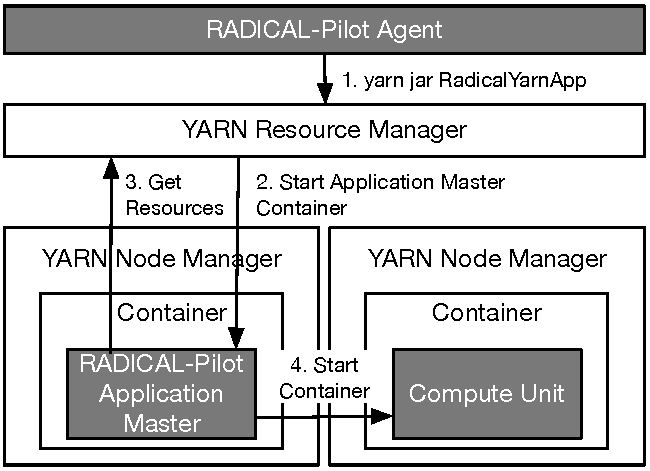
\includegraphics[width=.65\textwidth]{figures/data_analytics_hpc/hpc_hadoop/yarn.pdf}
    \caption{RADICAL-Pilot YARN Agent Application.}
%    \caption{\textbf{RADICAL-Pilot YARN Agent Application: }
%        RADICAL-Pilot provides a YARN application that manages the execution of Compute Units.
%        The application is initialized with parameters defined in the Compute Unit Description and started by the Task Spawner (step 1/2).
%        The Application Master requests resources from the Resource Manager and starts a container running the Compute Unit (step 3/4).}
    \label{fig:figures_yarn}
\end{figure}

\emph{RADICAL-Pilot Application Master:}
A particular integration challenge is the multi-step resource allocation process imposed by YARN depicted in Figure~\ref{fig:figures_yarn}, which differs significantly from HPC schedulers.
The central component of a YARN application is the Application Master, which is responsible for negotiating resources with the YARN Resource Manager as well as managing the execution of an application in the assigned resources.
The unit of allocation in YARN is a container~\cite{murthy2014apache}.
The YARN client (part of the YARN Launch Method) implements a YARN Application Master, which is the central instance for managing the resource requirements of an application.
RADICAL-Pilot utilizes a managed application master that is run inside a YARN container.
Once the Application Master container is started, it is responsible for requesting a YARN container meeting the resource requirements of the Compute Unit from the YARN's Resource Manager.
Once YARN allocates a set of containers, the CU starts inside these containers.
A wrapper script responsible for setting up a RADICAL-Pilot environment, staging of the specified files and running the executable defined in the Compute Unit Description, is used for this purpose.
Every Compute Unit is mapped to a YARN application consisting of an Application Master and a container of the size specified in the Compute Unit Description.

\subsubsection*{RADICAL-Pilot and Spark Integration}
\label{sssec:rp_spark}
Spark offers multiple deployment modes: standalone, YARN and Mesos.
While it is possible to support Spark on top of YARN, this approach is associated with significant complexity and overhead as two instead of one framework need to be configured and bootstrapped.
Since RADICAL-Pilot operates in user-space and single-user mode, no advantages with respect to using a multi-tenant YARN cluster environment exist.
Thus, we support Spark via the standalone deployment mode.

Similar to the YARN integration, the necessary changes for Spark are confined to the RADICAL-Pilot-Agent.
Similarly, the Local Resource Manager is responsible for initialization and deployment of the Apache Spark environment.
In the first step the LRM detects the number of cores, memory and nodes provided by the Resource Management System, verifies and downloads necessary dependencies (e.g., Java, Scala, and the necessary Spark binaries).
It then creates the necessary configuration files, e.g., \texttt{spark-env.sh}, \texttt{slaves} and \texttt{master} files, for running a multi-node, standalone Spark cluster.

Finally, the LRM starts the Spark cluster using the previously generated configuration.
Similar to YARN, a Spark RADICAL-Pilot-Agent scheduler is used for managing Spark resource slots and assigning CUs.
During the termination of the RADICAL-Pilot-Agent, the LRM is shutting down the Spark cluster using Spark’s termination script, which stops both the master and the slave nodes.
Similarly, the Spark specific methods for launching and managing Compute Units on Spark are encapsulated in a Task Spawner and Launch Method component.

\section{Experiments and Evaluation}
\label{sec:rph-exps}

To evaluate the RADICAL-Pilot YARN and Spark extension, we conduct two experiments.
In \S~\ref{ssec:startup_pilot_unit}, we analyze and compare RADICAL-Pilot and RADICAL-Pilot-YARN with respect to startup times of both the Pilot and the Compute Units.
We use the well-known K-Means algorithm to investigate the performance and runtime trade-offs of a typical data-intensive application, in \S~\ref{ssec:kmeans}.
Experiments are performed on two different XSEDE allocated machines: Wrangler~\cite{wrangler} and Stampede~\cite{stampede}.
On Stampede every node had 16 cores and 32 GB of memory; on Wrangler 48 cores and 128 GB of memory.
For our experiments we used RADICAL-Pilot v0.45, Hadoop v2.6 and Spark v2.0.2.

\subsection{Pilot Startup and Compute Unit Submission Characterization}
\label{ssec:startup_pilot_unit}

\begin{figure}[t]
    \centering
    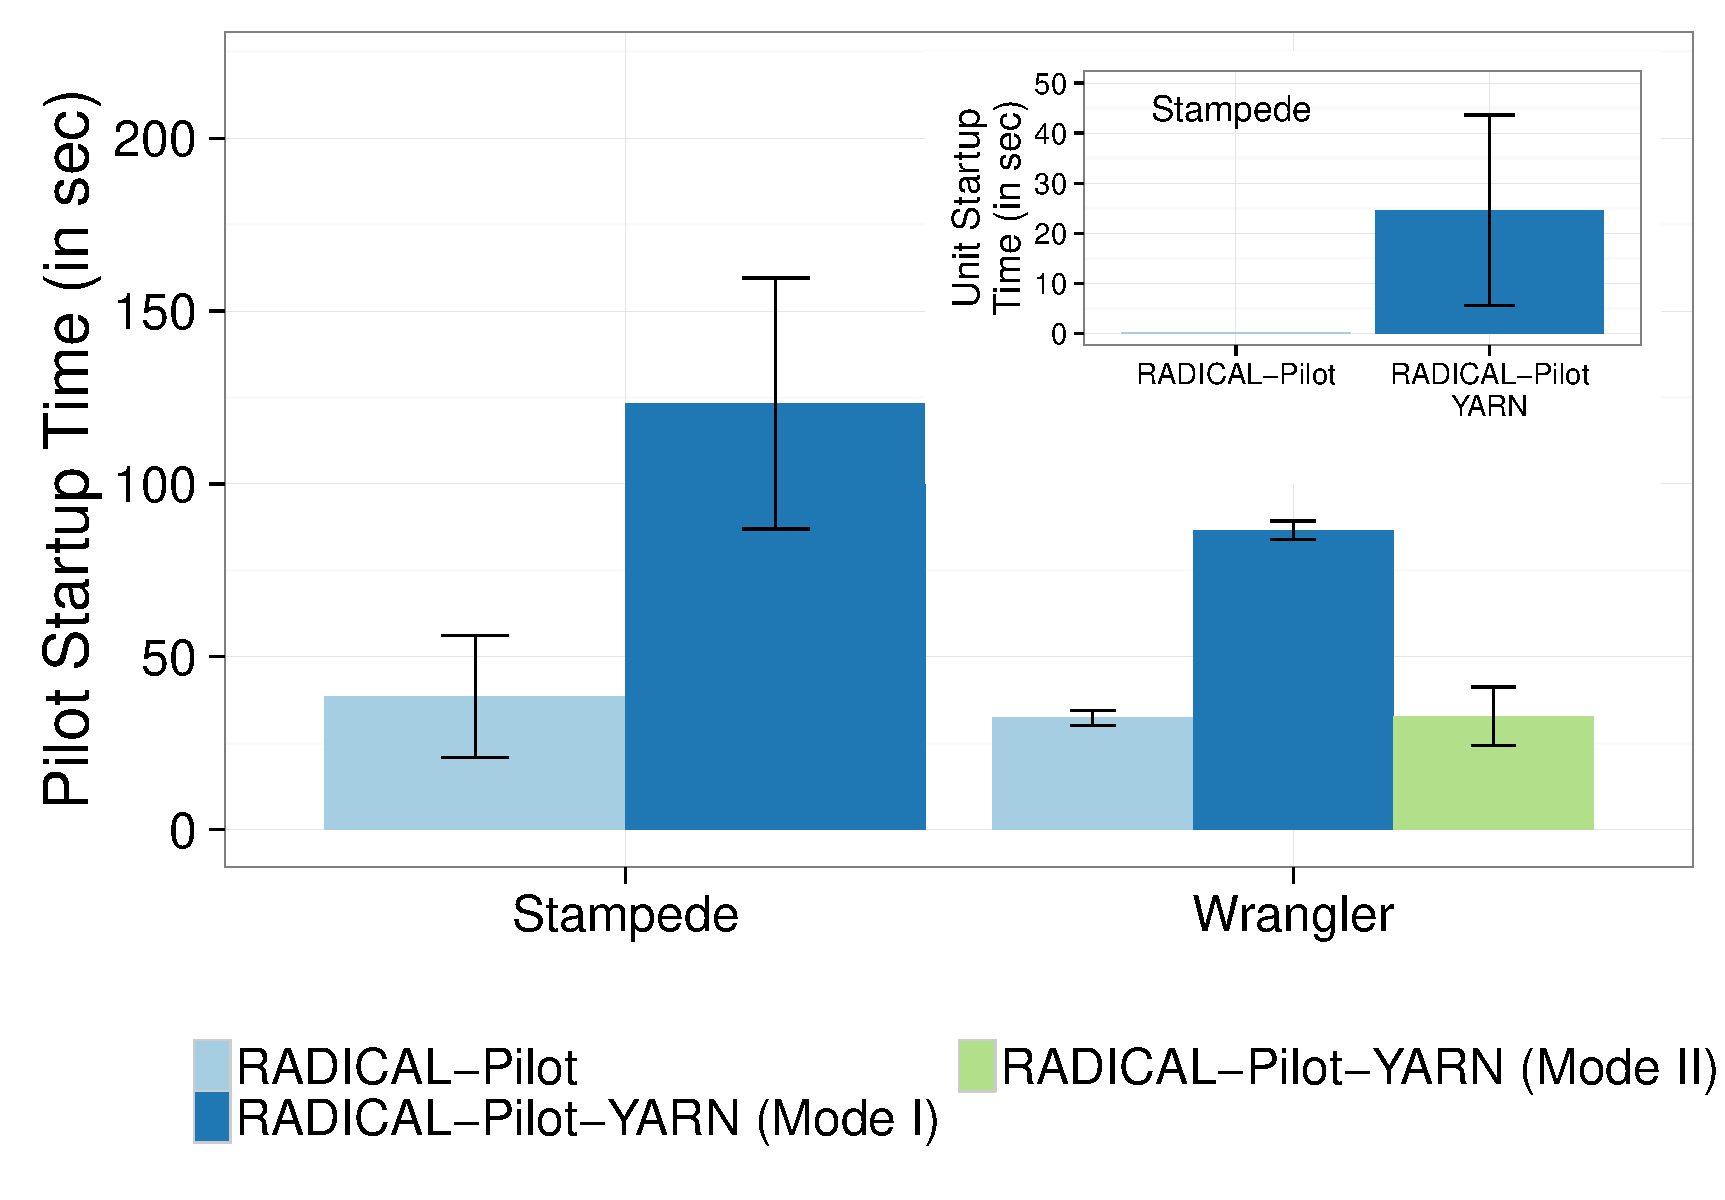
\includegraphics[width=0.75\textwidth]{figures/data_analytics_hpc/hpc_hadoop/pilot_unit_startup.pdf}
    \caption{RADICAL-Pilot and RADICAL-Pilot-YARN startup overheads.
        \label{fig:startup_yarn}}
%    \caption{\textbf{RADICAL-Pilot and RADICAL-Pilot-YARN startup overheads:}
%        The agent startup time is higher for YARN due to the overhead for spawning the YARN cluster.
%        The inset shows that the Compute Unit startup time (time between application submission to YARN and startup) is also significantly higher for YARN.
%        \label{fig:startup_yarn}}
\end{figure}

In Figure~\ref{fig:startup_yarn} we analyze the measured overheads when starting RADICAL-Pilot and RADICAL-Pilot-YARN, and when submitting Compute Units.
The agent startup time for RADICAL-Pilot-YARN is defined as the time between RADICAL-Pilot-Agent starts and the processing of the first Compute Unit.
On Wrangler, we compare both Mode I (Hadoop on HPC) and Mode II (HPC on Hadoop).
For Mode I the startup time is higher compared to the normal RADICAL-Pilot startup time and also compared to Mode II.
This can be explained by the necessary steps required tp download, configure and start the YARN cluster.
For a single node YARN environment, the overhead for Mode I (Hadoop on HPC) is between 50-85\,sec depending upon the resource selected.
The startup times for Mode II on Wrangler---using the dedicated Hadoop environment provided via the data portal---are comparable to the normal RADICAL-Pilot startup times as it is not necessary to spawn a Hadoop cluster.

The inset of Figure~\ref{fig:startup_yarn} shows the time taken to start Compute Units via RADICAL-Pilot to a YARN cluster.
For each CU, resources have to be requested in two stages: first the application master container is allocated followed by the containers for the actual compute tasks.
For short-running jobs this represents a bottleneck.

In summary, while there are overheads associated with executing inside of YARN, we believe these are acceptable, in particular for long-running tasks.
The novel capabilities of executing HPC tasks and YARN tasks within the same application has significant benefits for which measured overheads are likely acceptable.

\subsection{K-Means Performance Characterization}
\label{ssec:kmeans}
We compare the time to completion of the K-Means algorithm using two configurations: RADICAL-Pilot on HPC and RADICAL-Pilot in HPC/YARN mode. 
We use three different scenarios: 10,000 points and 5,000 clusters, 100,000 points / 500 clusters and 1,000,000 points / 50 clusters.
Each point belongs to a three dimensional space.
The compute requirements depend on the product of the number of points and clusters, thus it is constant for all three scenarios.
We use an optimized version of K-Means in which the sum and number of points are precomputed in the map phase, thus only these two attributes per cluster need to be shuffled.
The shuffle traffic depends on the number of clusters and decreases with the number of clusters.
For the purpose of this benchmark, we run two iterations of K-Means.

We utilize up to 3 nodes on Stampede and Wrangler.
Experiments are performed with the following configurations: 8 tasks on 1 node, 16 tasks on 2 nodes and 32 tasks on 3 nodes.
For RADICAL-Pilot-YARN, we use Mode II (Hadoop on HPC): the YARN Resource Manager is deployed on the node running the RADICAL-Pilot-Agent.

Figure~\ref{fig:experiments_kmeans_rpyarnkmeans} shows the results of executing K-Means over different scenarios and configurations.
For RADICAL-Pilot-YARN the runtimes include the time required to download and start the YARN cluster on the allocated resources.

\begin{figure}[t]
    \centering
    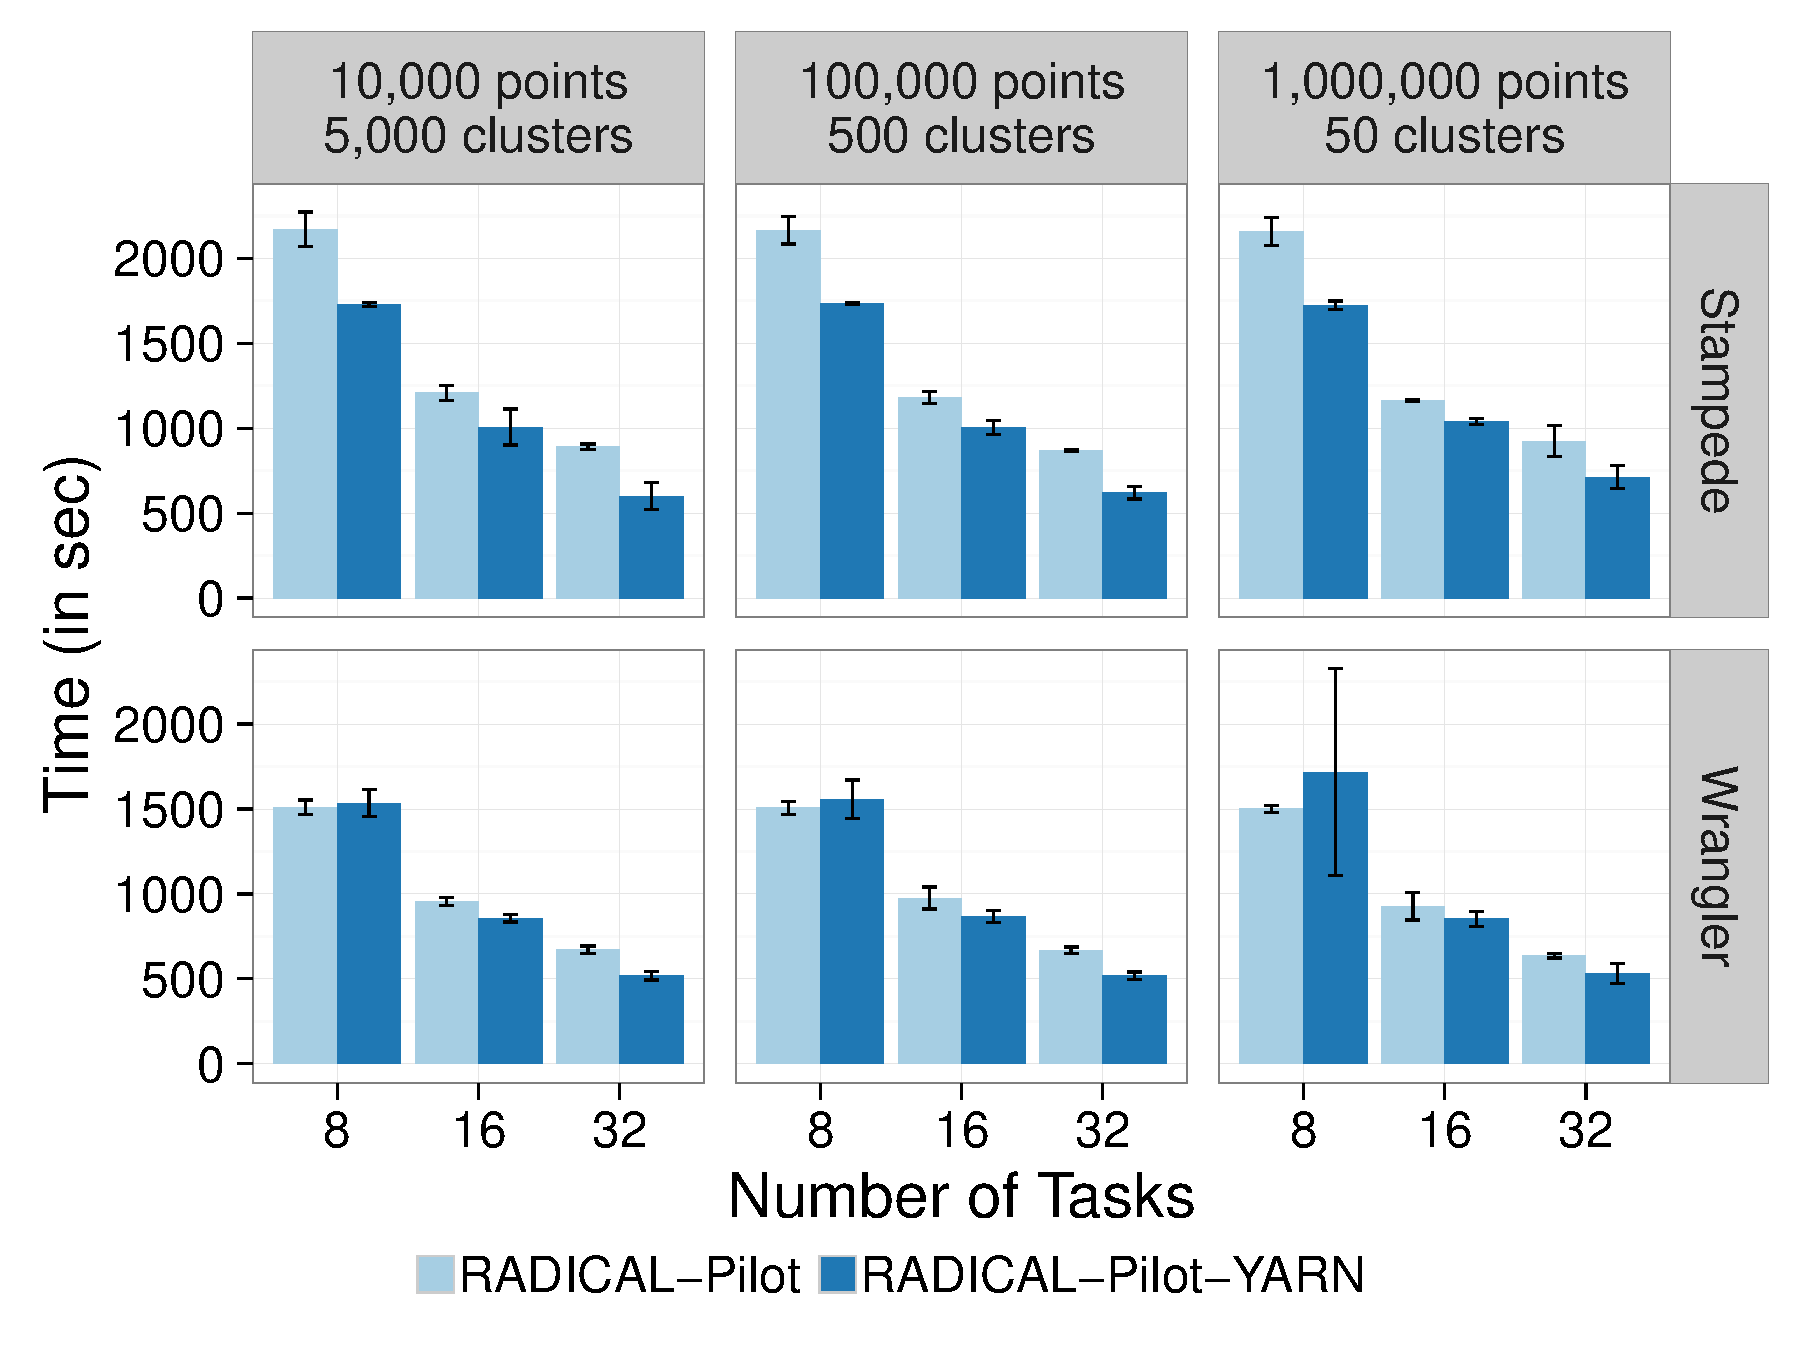
\includegraphics[width=.75\textwidth]{figures/data_analytics_hpc/hpc_hadoop/kmeans.pdf}
    \caption{RADICAL-Pilot and YARN-based K-Means time to completion on Stampede and Wrangler.}
%\caption{\textbf{RADICAL-Pilot and YARN-based K-Means on Stampede and Wrangler:}
%        Across all configurations the performance of the YARN backend is in average 13\,\% better.
%        On Wrangler a significant better performance and scalability (higher speedups) were observed.}
    \label{fig:experiments_kmeans_rpyarnkmeans}
\end{figure}

Independent of the scenario, the runtimes decrease with the number of tasks.
In particular, in the 8 task scenarios the overhead of YARN is visible on Wrangler.
For larger number of tasks, we observed on average 13~\% shorter runtimes for RADICAL-Pilot-YARN.
Also, RADICAL-Pilot-YARN achieves better speedups, e.\,g., 3.2 for 32 tasks for the 1 million points scenario, which is significantly higher than the RADICAL-Pilot speedup of 2.4 (both on Wrangler and compared to base case of 8 tasks).
One of the reasons is that for RADICAL-Pilot-YARN uses the local file system, while for RADICAL-Pilot uses the Lustre filesystem.

For similar scenarios and task/resource configuration, the runtimes on Wrangler show a significant performance improvements over Stampede.
This is attributed to the better hardware (CPUs, memory) of Wrangler than Stampede.
In particular for RADICAL-Pilot-YARN we observed on average higher speedups on Wrangler, indicating that we saturated the 32 GB of memory available on each Stampede node.

In summary, despite the overheads of RADICAL-Pilot-YARN with respect to Pilot and Compute Unit startup time, we were able to observe performance improvements (on average 13~\% better time to completion) mainly due to the better performance of the local disks.


\section{Conclusions}
\label{sec:hpc_hadoop_concl}

Hadoop and Spark are used by increasing number of scientific applications mainly due to accessible abstractions they provide.
HPC and Hadoop environments are converging, for example, MLLib/Spark utilize BLAS, Hadoop frameworks adopt parallel and in-memory computing concepts that originated in HPC.
Currently, traditional HPC applications lack the ability to access and use Hadoop and other Hadoop tools, without sacrificing the advantages of HPC environments.
One prominent reason behind the limited uptake, is finding effective and scalable resource management techniques usable for Hadoop frameworks on HPC infrastructure.

This chapter motivates the use of the Pilot-Abstraction as an integrating concept, discusses the design and implementation of RADICAL-Pilot extensions for Hadoop and Spark, and validates them with scalability analysis on two supercomputers.
Our experiments use RADICAL-Pilot, and introduce two extensions to RADICAL-Pilot to better integrate Hadoop on HPC.
We demonstrate that the Pilot-Abstraction strengthens the state of practice in utilizing HPC resources in conjunction with emerging Hadoop frameworks by allowing users to combine a diverse set of best-of-breed tools running on heterogeneous infrastructure consisting of HPC.
Using these capabilities, complex data campaigns can utilize a diverse set of Hadoop and HPC frameworks enabling scalable data ingests and analytics workflows.
Providing both a unifying and powerful abstraction that enables all parts of such a data pipeline to co-exist is critical.

While we demonstrated the importance of integrated capabilities for supporting data analytics on HPC, we want to understand their performance impact on scientific task-based data analytics scientific workflows.
This is important when executing computational campaigns on HPC resources, as selecting a suitable capability to execute data-intensive workflows is desirable.
Thus, we continue our work with integrating and measuring the performance of molecular dynamics data-analysis workflows utilizing these capabilities on HPC resources.

%%%%%%%%%%%%%%%%%%%%%%%%%%%%%%%%%%%%%%%%%%%%%%%%%%%%%%%%%%%%%%%%%%%%%%%%%%%%%%%%
%
%For example, Cray's analytics platform Urika~\footnote{http://www.cray.com/products/analytics} has Hadoop and Spark running on HPC architecture as opposed to regular clusters, but without the HPC software environment and capabilities.
%However, several applications ranging from bio-molecular simulations to epidemiology models~\cite{network1} require significant simulations interwoven with analysis capabilities such as clustering and graph analytics; in other words some stages (or parts of the same stage) of an application would ideally utilize Hadoop/Spark environments and other stages (or parts thereof) utilize HPC environments.
%
%Over the past decades, the High Performance Distributed Computing (HPDC) community has made significant advances in addressing resource and workload management on heterogeneous resources.
%For example, the concept of multi-level scheduling~\cite{1392910} as manifested in the decoupling of workload assignment from resource management using the concept of intermediate container jobs (also referred to as \pilotjobs~\cite{pstar12}) has been adopted for both HPC and Hadoop.
%Multi-level scheduling is a critical capability for data-intensive applications as often only application-level schedulers can be aware of the localities of the data sources used by a specific application.
%This motivated the extension of the \pilot-Abstraction to \pilotdata~\cite{pilot-data-jpdc-2014} to form the central component of a resource management middleware.
%
%In the following sections, we discuss a set of tools for supporting both of these usage modes:
%In section~\ref{ssec:saga_hadoop} we present SAGA-Hadoop, a light-weight tool for running Hadoop on HPC (Mode I).
%We then discuss, the integration of Hadoop and Spark runtimes into RADICAL-Pilot, which enables both the interoperable use of HPC and Hadoop, as well as the integration of HPC and Hadoop applications (Mode I and II) (Section~\ref{ssec:rp-impl}).
%Using these new capabilities, applications can seamlessly connect HPC stages (e.g., simulation stages) with analysis staging using the Pilot-Abstraction to provide unified resource management.
%
%\subsection{Mode I: SAGA-Hadoop, supporting Hadoop/Spark on HPC}
%\label{ssec:saga_hadoop}
%
%SAGA-Hadoop~\cite{saga-hadoop} is a tool for supporting the deployment of Hadoop and Spark on HPC resources (Mode I in Figure~\ref{fig:figures_hadoop-on-hpc-viceverse}).
%Using SAGA-Hadoop an applications written for YARN (e.g., MapReduce) or Spark (e.\,g. PySpark, DataFrame and MLlib applications) can be executed on HPC resources.
%
%Figure~\ref{fig:saga-hadoop} illustrates the architecture of SAGA-Hadoop.
%SAGA-Hadoop uses SAGA~\cite{merzky2015saga} to spawn and control Hadoop clusters inside an environment managed by an HPC scheduler.
%SAGA is used for dispatching a bootstrap process that generates the necessary configuration files and starting Hadoop.
%The specifics of the Hadoop framework (i.e., YARN and Spark) are encapsulated in a Hadoop framework plugin (also referred to as adaptors).
%SAGA-Hadoop delegates tasks, such as the download, configuration and start of a framework to this plugin.
%In the case of YARN, the plugin is then responsible for launching YARN's Resource and Node Manager processes; in the case of Spark, the Master and Worker processes.
%This architecture is extensible as new frameworks, e.g., Flink, can easily be added.
%
%\begin{figure}[t]
%    \centering
%    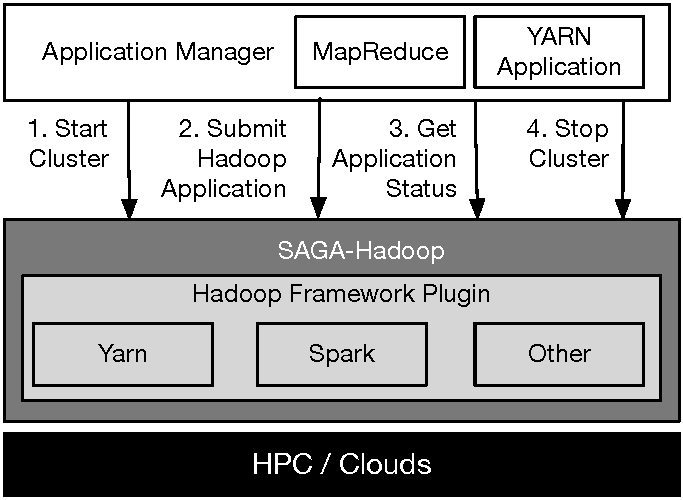
\includegraphics[width=.95\textwidth]{figures/data_analytics_hpc/hpc_hadoop/pilot-abds.pdf}
%    \caption{SAGA-Hadoop for HPC and Cloud Infrastructures.}
%    \label{fig:saga-hadoop}
%\end{figure}
%
%While nearly all Hadoop frameworks (e.g., MapReduce and Spark) support YARN for resource management, Spark provides a standalone cluster mode, which is more efficient in particular on dedicated resources.
%Thus, a special adaptor for Spark is provided.
%Once the cluster is setup, users can submit applications using SAGA's API that allows them to start and manage YARN or Spark application processes.
%
%While SAGA-Hadoop provides the interoperability between YARN and HPC resources by treating YARN as a substitute for common HPC schedulers, the integration of YARN and HPC applications or application stages remains challenging.
%As a consequence, we explored the usage of the Pilot~-Abstraction~\cite{luckow2012pstar}, through RADICAL-Pilot~\cite{merzky2019using}, to enable the integration between these different application types.